\pagebreak

\section{Decay-function integrals and inverse cumulative masses} \label{app:maths}
\subsection{Decay-function integrals} \label{app:integrals}
\subsubsection{Omori--Utsu} 

Using the substitution $u = 1 + \tau/c$, $\mathrm{d}u = \mathrm{d}\tau/c$,
\begin{equation*}
G_{\mathrm{OU}}(v,w) = \int_v^w g_{\mathrm{OU}}(\tau)\,\mathrm{d}\tau = c \int_{1+v/c}^{1+w/c} u^{-p}\,\mathrm{d}u
= \frac{c}{p-1}\Big[\big(1+\tfrac{v}{c}\big)^{1-p} - \big(1+\tfrac{w}{c}\big)^{1-p}\Big].
\end{equation*}
The antiderivative $u^{1-p}/(1-p)$ requires $p \neq 1$. Letting $v = 0$ and $w \to \infty$, the second term vanishes only for $p > 1$, giving the total mass $G_{\mathrm{OU}}(0,\infty) = c/(p-1)$; for $p \leq 1$, the integral diverges, as noted in Section~\ref{sec:ou}.


\subsubsection{Modified stretched exponential}
Using the substitution $u = (d+\tau)^{\gamma}$, $\mathrm{d}u = \gamma (d+\tau)^{\gamma - 1}\,\mathrm{d}\tau$,
\begin{align*}
G_{\mathrm{MSE}}(v,w) = \int_v^w g_{\mathrm{MSE}}(\tau)\,\mathrm{d}\tau
&= \frac{d^{\,1-\gamma}\exp(\rho d^{\gamma})}{\gamma} \int_{(d+v)^{\gamma}}^{(d+w)^{\gamma}} \exp(-\rho u)\,\mathrm{d}u \\
&= \frac{d^{\,1-\gamma}}{\rho\gamma}\Big[\exp\big\{-\rho\big[(d+v)^{\gamma} - d^{\gamma}\big]\big\} - \exp\big\{-\rho\big[(d+w)^{\gamma} - d^{\gamma}\big]\big\}\Big].
\end{align*}
Since $\rho, \gamma > 0$, letting $v = 0$ and $w \to \infty$ gives the total mass $G_{\mathrm{MSE}}(0,\infty) = d^{\,1-\gamma}/(\rho\gamma)$.

\subsubsection{Rate-state}
Using the substitution $u = \exp(-\tau/t_a)$, $\mathrm{d}u = -(u/t_a)\,\mathrm{d}\tau$,
 \begin{equation*}
 G_{\mathrm{RS}}(v,w) = \int_v^w g_{\mathrm{RS}}(\tau)\,\mathrm{d}\tau
= \frac{(1-B)\,t_a}{B} \int_{e^{-w/t_a}}^{e^{-v/t_a}} \frac{B}{1 - B u}\, \mathrm{d}u
= \frac{(1-B)\, t_a}{B}\, \log\left(\frac{1 - B e^{-w/t_a}}{1 - B e^{-v/t_a}}\right).
\end{equation*}
Here, $\log$ denotes the natural logarithm. Since $0 < B < 1$, letting $v = 0$ and $w \to \infty$ gives the total mass $G_{\mathrm{RS}}(0,\infty) = -(1-B)\,t_a\log(1-B)/B$.

\subsection{Inverse cumulative masses} \label{app:inverse}

Writing $C_k(\tau)=G_k(0,\tau)$, inversion of $C_k(\tau)=\omega$ gives
\begin{subequations}\label{eq:app-inverse-mass}
\begin{align*}
C_{\mathrm{OU}}^{-1}(\omega)
&=
c\left[
\left(
1-\frac{p-1}{c}\omega
\right)^{1/(1-p)}
-1
\right],
\\
C_{\mathrm{MSE}}^{-1}(\omega)
&=
\left[
d^\gamma
-\frac{1}{\rho}
\log\left(
1-\rho\gamma d^{\gamma-1}\omega
\right)
\right]^{1/\gamma}
-d,
\\
C_{\mathrm{RS}}^{-1}(\omega)
&=
-t_a
\log\left[
\frac{
1-(1-B)\exp\left\{
\frac{B\omega}{t_a(1-B)}
\right\}
}{B}
\right].
\end{align*}
\end{subequations}

\section{Figures} \label{app:figs}
\subsection{Simulation results} \label{app:synth}
\subsubsection{Posterior recovery under correct specification} \label{app:posterior-recovery}
 \begin{figure} [H]
    \centering
    
\includegraphics[width=0.9\linewidth]{images/parameter_posterior_overlays.pdf}
    \caption{Posterior parameter recovery under correct specification. Grey curves show posterior marginal densities across 100 synthetic catalogues; dashed lines mark generating values. OU denotes Omori--Utsu, MSE modified stretched exponential, and RS rate-state.}
    \label{fig:simulation-posteriors}
\end{figure}

\subsubsection{Posterior dependence under correct specification} \label{app:posterior-correlation}

\begin{figure} [H]
    \centering
    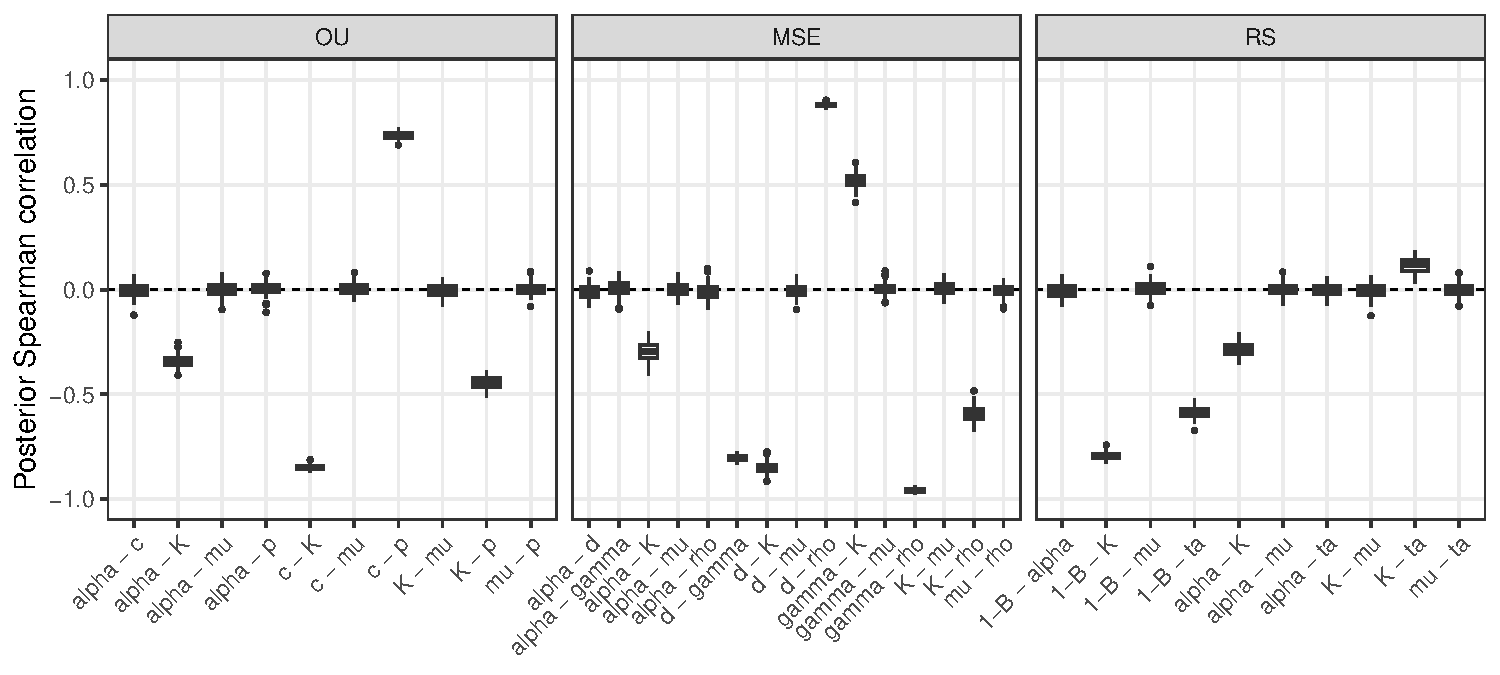
\includegraphics[width=0.9\linewidth]{images/posterior_parameter_correlations.pdf}
    \caption{Posterior dependence among ETAS parameters under correct specification. Boxplots show the distribution of within-catalogue posterior Spearman correlations across $100$ synthetic catalogues for each temporal form. Correlations are calculated from $1{,}000$ joint posterior samples per fitted catalogue. OU denotes Omori--Utsu, MSE modified stretched exponential, and RS rate-state.}
    \label{fig:simulation-posterior-correlation}
\end{figure}

\subsubsection{Posterior functional similarity under misspecification}\label{app:posterior-functional-tv}

\begin{figure} [H]
    \centering
    
\includegraphics[width=0.5\linewidth]{images/posterior_functional_tv.pdf}
    \caption{Posterior TV distance from the generating function across synthetic catalogues. Points show posterior medians, with bars indicating $95 \%$ credible intervals across $1{,}000$ joint posterior draws.}
    \label{fig:posterior-functional-tv}
\end{figure}
